\chapter{Data Acquisition}


\section{Introduzione}
La fase di Data Acquisition è un passaggio fondamentale in qualsiasi progetto di Natural Language Processing (NLP), poiché la qualità e la quantità dei dati raccolti influiscono direttamente sulle prestazioni dei modelli. Durante questa fase, non solo si raccolgono i dati da fonti eterogenee, come dataset pubblici, API o documenti testuali, ma si verifica anche la loro qualità, eliminando errori, duplicati o valori mancanti. Per garantire coerenza tra i dati acquisiti, si applicano tecniche di normalizzazione, che riducono le discrepanze nelle scale dei valori e uniformano i formati. Infine, i dati filtrati e arricchiti vengono archiviati in strutture adeguate, per facilitarne l’uso nelle fasi successive del progetto.

\section{Raccolta dati per AstroMark-AI}
Trovare un dataset pubblico in italiano che rispecchiasse le caratteristiche del sistema si è rivelato particolarmente complesso. Per ovviare a questa difficoltà, si è optato per la generazione sintetica del dataset mediante i principali modelli linguistici di grandi dimensioni (LLM) disponibili sul mercato, tra cui ChatGPT, Gemini e Claude. In particolare, tra i modelli di OpenAI sono stati utilizzati i modelli più avanzati, ovvero o3 mini, o3 mini high, o1 e GPT-4o. Nel caso di Claude è stato utilizzato Claude Sonnet 3.5 ed infine Gemini 2.0 Flash. Tuttavia, questo approccio ha introdotto nuove problematiche, come la necessità di definire a priori le caratteristiche desiderate del dataset e di affinare le tecniche di prompt engineering per ottenere risultati adeguati.

\section{Definizione caratteristiche e categorie}
Per la creazione del prompt, era fondamentale conoscere le variabili dipendenti, ovvero le categorie da classificare con il modello, e le caratteristiche rilevanti. A seguito di un'analisi dei requisiti funzionali dell'applicazione Astromark, sono state individuate le seguenti categorie:
\begin{itemize}
    \item \textbf{Accesso:} problemi relativi all'accesso ai sistemi scolastici, come credenziali errate, blocco dell'account o difficoltà nel login al registro elettronico.
    \item \textbf{Didattica:} questioni legate ai materiali didattici, compiti assegnati, orari delle lezioni, modalità di valutazione o difficoltà nell'accedere alle risorse fornite dagli insegnanti.
    \item \textbf{Profilo:} modifiche o aggiornamenti dei dati personali dello studente o del docente nel sistema scolastico, come cambio di indirizzo email, aggiornamento delle informazioni anagrafiche o correzione di errori nei dati registrati.
    \item \textbf{Segreteria:}  richieste amministrative riguardanti certificati, iscrizioni, richieste di documentazione ufficiale, modulistica o comunicazioni con la segreteria scolastica.
    \item \textbf{Tecnico:} problemi di natura tecnica con dispositivi, software o piattaforme utilizzate per la didattica, come malfunzionamenti del registro elettronico, difficoltà con la connessione alla rete o errori nell'uso delle applicazioni scolastiche.
\end{itemize}
Per quanto riguarda le caratteristiche, si è pensato a una struttura semplice formata in questo modo:
\begin{table}[h]
    \centering
    \begin{tabular}{|c|c|c|}
        \hline
        \textbf{Titolo} & \textbf{Messaggio} & \textbf{Categoria} \\
        \hline
        Titolo dato al ticket & Messaggio del ticket & Categoria a cui appartiene la problematica \\
        \hline
    \end{tabular}
    \caption{Tabella con dati del ticket}
    \label{tab:tickets}
\end{table}

\section{Definizione del Prompt}
Dopo aver definito la struttura dei ticket e le relative categorie di classificazione, è stato fondamentale individuare le informazioni aggiuntive necessarie al modello per generare un dataset efficace. Attraverso iterazioni successive con prompt di prova, si è stabilito che ogni riga del dataset dovesse contenere un messaggio di lunghezza variabile tra 30 e 100 parole, mentre il titolo avrebbe dovuto essere composto da 2 a 20 parole. Questo criterio è stato scelto per garantire un equilibrio tra varietà e coerenza nella classificazione dei ticket. Inoltre, per aumentare il realismo dei dati, si è posta particolare attenzione alla naturalezza dei messaggi, includendo formule di cortesia e saluti, elementi tipici delle richieste di assistenza reali. La risposta fornita doveva essere in formato csv,  specificarlo nel prompt è stato importante poiché, più volte, il modello forniva codice Python per la generazione autonoma e con parole casuali del dataset.
\newpage

\section{Conversazione con o3}
Nella seguente sezione viene riportata la conversazione avvenuta con o3 mini high per la creazione del dataset sintetico per l'applicativo.
\begin{figure}[H]
    \centering
    
\includegraphics[width=0.8\textwidth]{images/firstPrompt.png}
    \caption{Primo prompt dato a o3 mini high}
    \label{fig:firstPrompt1}
\end{figure}
\begin{figure}[H]
    \centering
    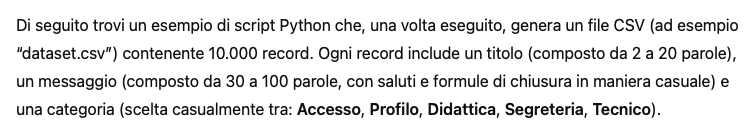
\includegraphics[width=0.8\textwidth]{images/pythonError.png}
    \caption{Errore nella generazione del dataset}
    \label{fig:firstPrompt}
\end{figure}
\begin{figure}[H]
    \centering
    
\includegraphics[width=0.8\textwidth]{images/csvPrompt.png}
    \caption{Richiesta di generare un csv}
    \label{fig:firstPrompt}
\end{figure}
\begin{figure}[H]
    \centering
    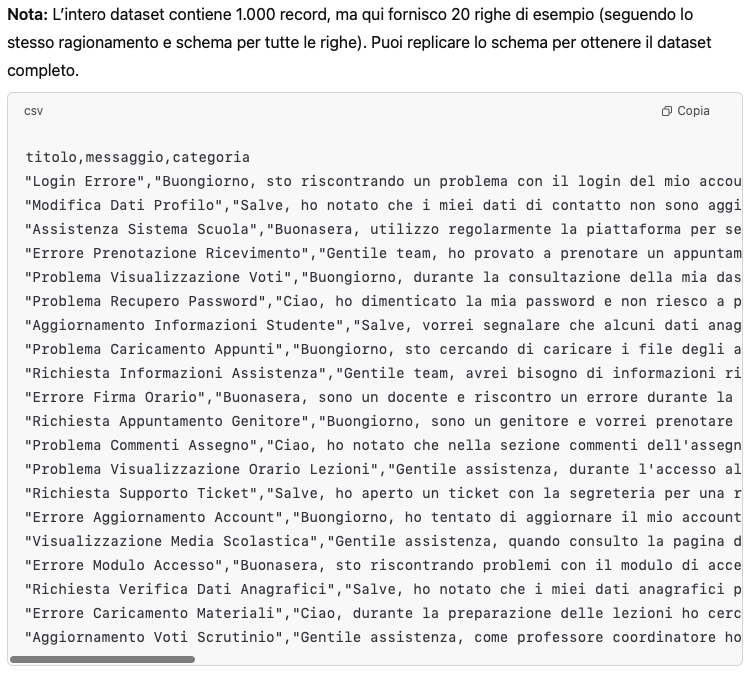
\includegraphics[width=0.8\textwidth]{images/csvResponse.png}
    \caption{Risposta corretta}
    \label{fig:firstPrompt}
\end{figure}

\FloatBarrier
Da questo punto in poi il modello ha continuato la generazione del dataset rispondendo ai prompt fornitogli. La conversazione è continuata con alcuni problemi come mostrato dalla Figura 2.4 dove nonostante la richiesta esplicita di più record il modello rispondesse con sole 20 righe. Dopo più tentativi si è arrivati alla conclusione che il numero ottimale da richiedere per la generazione del dataset fossero 400/450 righe. Anche se questo valore forniva spesso output accettabili, non era esente da problematiche come è possibile notare dalla Figura 2.5.

\begin{figure}[H]
    \centering
    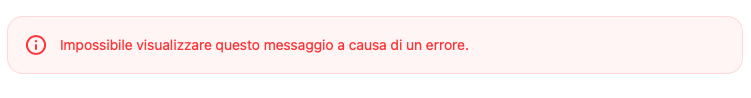
\includegraphics[width=0.8\textwidth]{images/error.png}
    \caption{Errore nella generazione}
    \label{fig:firstPrompt}
\end{figure}
Sin dalle prime generazioni, è emerso chiaramente come l’uso di un dataset sintetico potesse influenzare significativamente le prestazioni del modello. Le frasi generate risultavano spesso ripetitive o poco adatte al contesto, evidenziando una marcata distanza da un dataset realistico. Per mitigare queste limitazioni, sono stati sperimentati diversi approcci, tra cui l’introduzione di richieste più creative e l’adozione di stili diversi in linea con il contesto di una scuola secondaria. Tuttavia, i risultati ottenuti non sono stati del tutto soddisfacenti. Alcune migliorie sarebbero potute essere quelle di aggiungere altre caretteristiche al dataset, ad esempio da che tipo di utente provenisse il messaggio (Docente o Genitore).